% Metódy inžinierskej práce

\documentclass[10pt,twoside,slovak,a4paper]{article}

\usepackage[slovak]{babel}
\usepackage{pdfpages}
%\usepackage[T1]{fontenc}
\usepackage[IL2]{fontenc} % lepšia sadzba písmena Ľ než v T1
\usepackage[utf8]{inputenc}
\usepackage{graphicx}
\usepackage{url} % príkaz \url na formátovanie URL
\usepackage{hyperref} % odkazy v texte budú aktívne (pri niektorých triedach dokumentov spôsobuje posun textu)



\usepackage{cite}
%\usepackage{times}

\pagestyle{plain}

\title{Kvízová hra, ako moderný predajný nástroj\thanks{Semestrálny projekt v predmete Metódy inžinierskej práce, ak. rok 2022/23, vedenie: XY}} 


\author{Martin Vančo\\[2pt]
	{\small Slovenská technická univerzita v Bratislave}\\
	{\small Fakulta informatiky a informačných technológií}\\
	{\small \texttt{xvancom@stuba.sk}}
}


\date{\small 6. november 2022}

\begin{document}

\maketitle

\begin{abstract}
	S príchodom novej éry sociálnych sietí sa zmenila aj forma marketingu. Je oveľa jednoduchšie nájsť koncového zákazníka, no čoraz náročnejšie ho udržať. V tomto článku preskúmame gamifikáciu, jej klúčové koncepty a ukážeme si ako využiť jej princípy na zvýšenie interakcie s našími zákazníkmi. Ďalej Definujeme herné mechaniky, a ukážeme si ich využitie v rôznych sférach marketingu. Hlavnou témou bude vedomostný kvíz, ktorý sme vytvorili. Ten budeme analyzovať a vysvetlovať klúčové rozhodnutia pri procese jeho tvorby. Záverom článku bude analýza úspečnosti tejto metódy.
\end{abstract}
\clearpage

\section{Úvod}\label{uvod}

	S príchodom sociálnych médií naberá online marketing na popularite. Vďaka platenej propagácií na internete nebolo nájdenie koncových zákazníkov nikdy jednoduchšie. Vďaka tejto novej forme propagácie značky je čoraz náročnejšie svoje publikum udržať. Zákazníci sú neustále bombardovaní reklamami na podobný produkt ako ten náš, a je čím ďalej tým náročné si zákazníka pri tomto konkurenčnom boji udržať. To čo zákazníka skutočne udrží je vzťah a povedomie o značke. Preto sa stalo publikovanie relevantného obsahu na sociálne siete značky dôležitejšie ako kedykoľvek predtým.
	
	Jedným z typov obsahu, ktorým dokážu firmy zaujať či vytvoriť interakciu, sú súťaže, ,vernostné programy, kvízy, alebo hry. Jedná sa o obsah ktorý využíva prvky takzvanej “gamifikácie”. O tom, čo slovo gamifikácia znamená, ako sa v marketingu využíva a ako môžu byť prvky gamifikácie prospešné k budovaniu zákazníkov sa budeme venovať práve v tomto článku.


\section{Gamifikácia}\label{gamifikacia}
	Predtým ako si predstavíme pojem gamifikácia si potrebujeme ujasniť, čo vlastne slovo “hra” znamená. V knihe “What are game mechanics”  od D. Cooka \cite{WhatAreGameMechanics}, je hra definovaná ako “Systém založený na pravidlách, ktoré povzbudzujú používateľa, aby skúmal a objavoval svoje možnosti za pomoci mechanizmov okamžitej spätnej väzby”. Spätná väzba je v tomto prípade počet nazbieraných bodov, ukazovateľ počtu životov alebo aktuálny level. Tieto ukazatele podnecujú hráča, aby danú hru hral, až pokým sa nedostane k odmene buď fyzickej (darčekový predmet, pohár) alebo virtuálnej (predmety v hre, herná mena). 
	Na základe tohto tvrdenia môžeme definovať gamifikáciu ako aktivitu, pri ktorej je základná úloha rozšírená o pravidlá, ktoré poskytujú užívateľovi spätnú väzbu, a o mechanizmy interakcie, čo tvorí celkovú hodnotu pre používateľa. Tento princíp sa uplatňuje najmä vo vzdelávaní mládeže, kedy sú deti motivované sa vzdelávať prostredníctvom zábavnej činnosti zo snahou nazbierať čo najviac bodov, alebo súperiť s konkurenciou.



\section{Marketing}\label{marketing}

	V knihe “Marketing” od Churchilla je marketing rozdelený na dva aspekty. \cite{churchill2017marketing}Po prvé je to filozofia, postoj alebo perspektíva, ktorá kladie dôraz na zákazníkovu spokojnosť. Po druhé, to sú činnosti a procesy implementujúce túto filozofiu.
	Dobrý marketing tvorí základ úspešného produktu. Vraví sa, že dobrý nápad tvorí iba 5\% toho, čo potrebujeme na vytvorenie prosperujúcej firmy. Marketing sa zaoberá hlavne predajom produktu koncovým zákazníkom. Ide o kombináciu vizuálnych, alebo zvukových prvkov, ktoré v spojení s kreativitou majú presvedčiť zákazníka o kúpe práve nášho produktu. Týmito prvkami môže byť billboard, fotografia, plagát, reklama v televízií alebo na sociálnych sieťach, atď.


\section{Využitie gamifikácie v marketingu}\label{pouzitie-v-marketingu}
V dobe, kedy dominuje prevažne digitálny marketing je dôležité, aby si náš produkt zákazník pamätal. To docielmime tým, že o svojej značke budeme zvyšovať povedomie. V nasledujúcej časti článku sa budeme venovať rôznym stratégiam, ako gamifikáciu v marketingu využiť a čo môže danej firme priniesť. Taktiež sa pokúsime analyzovať ju z hľadiska definície herných mechaník.

\subsection{Súťaž zdieľaním}
Klasická veta “Pošli to trom kamarátom a vyhraj”. Určite sa mnohí z nás už do podobnej súťaže zapojili. Firma na svoje sociálne siete publikuje príspevok, v ktorom ohlási pravidlá zapojenia sa do súťaže. Pravidlá sú hneď prvým znakom herných mechaník. V tomto prípade ide o to, aby sa do súťaže zapojilo čo najviac ľudí. Preto je zapojenie sa do súťaže zväčša podmienené zdieľaním príspevku. Výhra je obvykle hmotná a dostatočne atraktívna na to, aby sa do súťaže zákazník zapojil. Odmena a konkurencia sú ďalšie aspekty ktoré potvrdzujú využitie prvkov gamifikácie. Na konci súťaže sa vylosuje náhodný výherca, ktorému bude cena odovzdaná. Takýto trik väčšinou slúži na zvýšenie počtu sledovateľov či záujemcov o produkt, čo potenciálne znamená aj zvýšenie predajov.

\subsection{Vedomostný kvíz}
Tento typ gamifikácie v marketingu využíva narozdiel od toho predchádzajúceho bodové ohodnotenie ako odmenu. Opäť sa však jedná o niečo, čo sa propaguje cez sociálne siete. Zvyčajne sa kvíz odohráva na webovej stránke danej firmy. Ďalší mechanizmus gamifikácie ktorý sa využíva je konkurencia. Porovnávanie sa s priateľmi o to, kto nazbieral viac bodov, kto zvládol kvíz za najkratší čas a podobne. Veľmi dôležitá je aj okamžitá spätná väzba. Súťažiaci vidí v reálnom čase počet nazbieraných bodov, a cieľom je ich nazbierať čo najviac. To motivuje súťažiaceho v niektorých prípadoch opakovať, čo zvyšuje interakciu.

\clearpage
\section{Použitie v praxi}
Počas letného festivalu Pohoda 2022 sme pre slovenský pivovar Urpiner vytvorili kvízovú hru s názvom S Urpinerom po Slovensku, ktorá mala otestovať použitie herných mechaník na zvýšenie interakcie medzi značkou a zákazníkom. Témou kvízu mali byť známe slovenské hrady, pamiatky, či pohoria.

Keďže sa jedná o značku, ktorá predáva pivo, bolo potrebné aby sa obsah čo najviac spájal s firemnou identitou. Princíp hry spočíval v tom, že súťažiaci mali priradiť názvy slovenských pamiatok ku každému z 18 obrázkov. Pre zatraktívnenie hry boli obrázky prekreslené do ilustrácií pivného pohára, v ktorého pene bola ukrytá hľadané pamiatky. Príklad toho, ako tieto ilustrácie vyzerali nájdete na obrázku nižšie.

\begin{figure}[h]
	\centering
	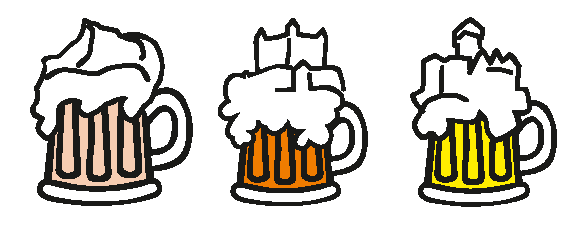
\includegraphics[scale=1.0]{obrazok1.pdf}

\caption{Ukážka ilustrácií použitých v kvíze}

\end{figure}


Rozhodli sme sa, že daná hra bude prebiehať v online podobe na webovej stránke spoločnosti. To nám umožnilo vytvoriť okamžitú spätnej väzby, v tomto prípade sa jednalo o vyhodnotenie kvízu po odoslaní správnych odpovedí. 

Veľmi klúčové bolo aj navrhnutie webovej stránky. Vzhľad musel byť jednoduchý, a pochopitelný. Celý proces vyplnenia kvízu prebiehal nasledovne:




\begin{enumerate}
	\item Návštevníci festivalu sa prostredníctvom QR kódov rozmiestnených po areále festivalu dostali na webovú stránku súťaže.
	\item Hráč sa následne presunul do sekcie s registráciou', kde zadal hráč svoje osobné údaje, konkrétne meno a emailovú adresu, čím sa úspešne zapojil do súťaže.
	\item Webová stránka stručne vysvetlila hráčovy pravidlá, postup vyplnenia odpovedí a následne sa spustil časový odpočet.
	\item Po vyplnení odpovedí stránka zobrazila získaný počet bodov a čas za ktorý súťažiaci kvíz vyplnil.
\end{enumerate}




Pre získanie ceny bol kľúčový počet nazbieraných bodov a čas. Podla týchto parametrov sa následne vybralo 9 najlepších súťažiacich, zoradených podľa získaného počtu bodov a času vyplnenia, ktorým sa ceny odovzdali.
\clearpage
\section{Výsledok kvízovej hry}

Hlavným cieľom celej súťaže bolo spríjemnenie festivalu účastníkom a taktiež zvýšenie povedomia o krásach Slovenska. Súťaže sa zúčastnilo celkom 698 súťažiacich, čo predstavuje približne 2,5\% konverziu (na festivale sa zúčastnilo približne 30 000 ľudí). Výsledky sú ale uspokojivé. Výsledkom kvízu je 700 nových potenciálnych zákazníkov, ktorých je možné osloviť prostredníctvom emailovej adresy ktorú zadali pri registrácií. Taktiež dúfame, že sme aspoň trochu poukázali na krásu Slovenska.

\bibliography{literatura}
\bibliographystyle{plain} 
\end{document}
